\documentclass[titlepage=firstcover, captions=tableheading]{scrartcl}
\usepackage{microtype}
\usepackage{amsmath}
\usepackage{polyglossia}
\usepackage{graphicx}
\usepackage{booktabs}
\usepackage{siunitx}
\usepackage{hyperref}
\usepackage{caption}
\usepackage{float}
\setdefaultlanguage{german}
\title{311 Der Hall-Effekt}
\author{
Connor Magnus Böckmann \\ email: \href{mailto:connormagnus.boeckmann@tu-dortmund.de}{connormagnus.boeckmann@tu-dortmund.de}
\and Tim Theissel \\ email: \href{mailto:tim.theissel@tu-dortmund.de}{tim.theissel@tu-dortmund.de}  
}
\begin{document}
\maketitle
\newpage
\tableofcontents
\newpage
\section{Zielsetzung}
Das Ziel des Versuchs 311 "Hall-Effekt und Elektrizitätsleitung bei Metallen" ist die Ermittlung der Leitfähigkeit einer Metallprobe anhand makroskopisch messbarer Parameter, wie etwa den geometrischen Abmessungen, der Hallspannung und dem Widerstand.

\section{Theoretische Grundlagen}
\subsection{Bandstruktur und Leitfähigkeit von Kristallen}
Kristalle bestehen aus Gittern, in denen die Atome so nah beieinander sind, dass sich ihre Valenzelektronen-die Außenelektronen-sich verhalten wie ein kontinuirliches System. Alle diese Elektronen unterliegen jedoch dem Pauli-Prinzip, welches besagt, dass keine zwei Elektronen im exakt gleichen Quantenzustand sein können. Das führt dazu, dass alle Elektronen unterschiedliche Energien besitzen. Im Unterschied zu den streng definierten Energieniveaus eines Einzelatoms, bilden sich hier also quasi kontinuierliche Energiebänder. Die Lücke zwischen zwei Energiebändern nennt man dabei verbotene Zone. Diese Energien können also nicht von Elektronen angenommen werden. Die Energiebänder können nur eine endliche Anzahl von Elektronen enthalten. Aufgefüllt werden die Energiebänder immer von den unteren Orbitalen zu den oberen Orbitalen. Elektronen aus vollbesetzten Bändern tragen nicht zur Leitfähigkeit bei, da sie keine Energie durch ein elektrisches Feld aufnehmen können. Ungepaarte Elektronen in nicht voll besetzten Energiebändern können sich in Richtung eines angelegten elektrischen Feldes bewegen. Ein makroskopischer elektrischer Strom entsteht. Die hohe elektrische Leitfähigkeit von Metallen resultiert also aus ihren nur teilweise besetzten oberen Energiebändern. Dieses wird Leitfähigkeitsband genannt. \\
Bei Isolatoren ist das oberste Energieband folglich leer und die verbotene Zone zu breit, um von Elektronen aus einem niedrigeren Band übersprungen zu werden. \\
Ein ideales Kristallgitter müsste nach der Quantentheorie eine unendlich hohe elektrische Leitfähigkeit besitzen, was aber auf Grund von Gitterbaufehlern nicht der Fall ist.
\subsection{Zur Berechnung der elektrischen Leitfähigkeit eines Metalles}
Die Leitungselektronen eines Metalls verhalten sich wie die Teilchen eines idealen Gases und stoßen beständig mit Strukturfehlern und Ionenrümpfen zusammen. Man kann nun die Zeit zwischen zwei Zusammenstößen mitteln und so die mittlere Flugzeit $\bar{\tau}$ erhalten. Wenn nun ein elektrisches Feld anliegt, werden die Elektronen während $\bar{\tau}$ gleichmäßig beschleunigt. Die Geschwindigkeitsänderung beträgt dann:
\begin{equation}
   \Delta \vec{\bar{v}}=-\frac{e_0}{m_0}\vec{E}\bar{\tau}
\end{equation}
Das Elektron wird dabei in eine zufällige Richtung gestreut. Im Mittel hat es also bei Beginn der Flugzeit die Geschwindigkeit 0 in Richtung des elektrischen Feldes. Daher kann eine mittlere Driftgeschwindigkeit $\vec{\bar{v_d}}$ eingeführt werden:
\begin{equation}
    \vec{\bar{v_d}}=\frac{1}{2}\Delta\vec{\bar{v}}
\end{equation}
Wenn nun ein elektrischer Leiter n Elektronen pro Volumeneinheit enthält und sich diese mit $\vec{\bar{v_d}}$ in Richtung von $\vec{E}$ bewegen, ist die Stromdichte j:
\begin{equation}
    j=-n\bar{v_d}e_0
\end{equation}
Dabei kann man $\bar{v_d}$ durch (?) und (?) ausdrücken.
\begin{equation}
    j=\frac{1}{2}\frac{e_0^2}{m_0}n\bar{\tau}E
\end{equation}
Es wird ein homogener Leiter (Länge L und Querschnitt Q) angenommen, weshalb j durch I/Q und E durch U/L ersetzt werden können.
\begin{equation}
    I=\frac{1}{2}\frac{e_o^2}{m_0}n\bar{\tau}\frac{Q}{L}U
\end{equation}
Der hier dargestellte Proportionalitätsfaktor zwischen der Spannung und Strom ist die elektrische Leitfähigkeit S:
\begin{equation}
    S=\frac{1}{2}\frac{e_o^2}{m_0}n\bar{\tau}\frac{Q}{L}
\end{equation}
Das Reziproke zur Leitfähigkeit ist der elektrische Widerstand R:
\begin{equation}
    R=2\frac{m_0}{e_0^2}\frac{1}{n\bar{\tau}}\frac{L}{Q}
\end{equation}
Daraus ergeben sich die geometrieunabhängigen Werte der spezifischen Leitfähigkeit \sigma und des spezifischen Widerstands\rho:
\begin{equation}
    \sigma=\frac{1}{2}\frac{e_o^2}{m_0}n\bar{\tau}
\end{equation}

\begin{equation}
    \rho=2\frac{m_0}{e_0^2}\frac{1}{n\bar{\tau}}
\end{equation}
Der Widerstand lässt sich leicht und relativ präzise an einem Draht messen. Die Gleichung enthält aber weiterhin mikroskopische Größen-n und $\bar{\tau}$. Daher werden weitere Zusammenhänge zwischen mikroskopischen Größen und makroskopisch messbaren Parametern benötigt.

\subsection{Der Hall-Effekt}
Im folgenden wird sich auf den in Abb.1 gezeigten Versuchsaufbau bezogen und die Bezeichnungen daraus verwendet. \\
\begin{figure}[H]
    \centering
    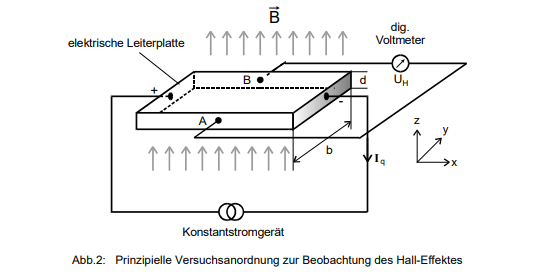
\includegraphics[height=9cm]{Versuchsanordnung_HallEffekt.png}
    \captionbelow{Prinzipielle Versuchsanordnung zur Beobachtung des Hall-Effektes}
\end{figure}
An eine homogene Leiterplatte, die Probe, der Dicke d und der Breite b wird der Länge nach ein konstanter Strom I\textsubscript{q} angelegt. An den Punkten A und B kann dann eine so genannte Hallspannung gemessen werden, wenn dann die Probe noch senkrecht zur Stromrichtung von I\textsubscript{q} von einem homogenen Magnetfeld $\vec{B}$ durchsetzt wird. Diese entsteht auf Grund der Lorentzkraft $\vec{F\textsubscript{L}}$, welche auf die Elektronen wirkt und diese ablenkt.
\begin{equation}
    F_L=e_0\vec{\bar{v_d}}B
\end{equation}
Sie zeigt dabei in negative y-Richtung wegen der negativen Ladung der Elektronen. Dadurch erhalten die Elektronen eine Geschwindigkeit in y-Richtung, woduch ein weiteres E-Feld entsteht, welches als $\vec{E\textsubscript{y}}$ der Bewegung in y-Richtung entgegen wirkt. $\vec{E\textsubscript{y}}$ wird dabei genau so groß, dass es die Lorentzkraft aufhebt.
\begin{equation}
    e_0E_y=e_0\vec{\bar{v_d}}B
\end{equation}
Die Hallspannung berechnet sich dann zu:
\begin{equation}
    U_H=E_y*b=\vec{\bar{v_d}}B*b
\end{equation}
$\vec{\bar{v_d}}$ lässt sich dabei durch den Querstrom I\textsubscript{q}:
\begin{equation}
    j=\frac{I_q}{b*d}=-ne_0\vec{\bar{v_d}}
\end{equation}
Also gilt:
\begin{equation}
    U_H=-\frac{1}{ne_0}\frac{B*I_q}{d}
\end{equation}
Die benötigte Ladungsträgerdichte n errechnet sich also nach:
\begin{equation}\label{Ladungsträger n}
    n=-\frac{1}{U_He_0}\frac{B*I_q}{d} 
\end{equation}
Mit bekanntem n lässt sich nun die mittlere Flugzeit $\bar{\tau}$ berechnen:
\begin{equation}
    \bar{\tau}=2\frac{m_0}{e_0^2}\frac{1}{nR}\frac{L}{Q}
\end{equation}
Außerdem lässt sich $\vec{\bar{v_d}}$ nun bestimmen:
\begin{equation}
    \vec{\bar{v_d}}=\frac{I}{-nQe_0}
\end{equation}
\subsection{Weitere Leitfähigkeitsparameter aus R und U\textsubscript{H}}
Der nächste zu bestimmende Parameter ist die mittlere freie Weglänge $\bar{l}$. Sie stellt die Entfernung, die ein Leitungselektron im Mittel zwischen zwei Zusammenstößen im Kristall zurücklegt. Sie errechnet sich nach:
\begin{equation}
    \bar{l}=\bar{\tau}*\mid v\mid
\end{equation}
\mid v\mid stellt dabei die Totalgeschwindigkeit der Elektronen dar. Da diese, wie bereits oben beschrieben wurde, dem Pauli-Verbot unterliegen, gilt nicht die klassische Maxwell-Boltzmann-Statistik. Viel mehr lässt sich zeigen, dass Elektronen der Fermi-Dirac-Verteilung unterliegen:
\begin{equation}
    f(E)=\frac{1}{e^\frac{E*E_F}{kT}+1}dE
\end{equation}
Die Fermi-Energie E\textsubscript{F} errechnet sich zu:
\begin{equation}
    E_F=\frac{h^2}{2m_0}\sqrt[3]{(\frac{3}{8\pi}n)^2}
\end{equation}
h stellt dabei das Planksche Wirkungsquantum dar. Im Wesentlichen hängt E\textsubscript{F} von der Dichte der Elektronen im Festkörper ab. Nur die wenigen Elektronen mit E\approx E\textsubscript{F} sind verantwortlich für die Leitfähigkeit des Metalls, da diese Energie aus einem äußeren E-Feldes aufnehmen können. Daraus folgt für $\mid \bar{v} \mid$:
\begin{equation}
    \mid \bar{v} \mid\approx \sqrt{\frac{2E_F}{m_0}}
\end{equation}
Für die gesuchte freie Weglänge ergibt sich daraus:
\begin{equation}
    \bar{l}\approx\bar{\tau}\sqrt{\frac{2E_F}{m_0}}
\end{equation}
Außerdem lässt sich die mikroskopische Größe der Beweglichkeit \mu der Ladungsträger bestimmen. Sie ist definiert als Verhältnis zwischen Driftgeschwindigkeit $\vec{\bar{v_d}}$ und der äußeren Feldstärke.
\begin{equation}
    \vec{\bar{v_d}}=\mu\vec{E}
\end{equation}
\begin{equation}
    \mu=\frac{1}{2}\frac{e_0}{m_0}*\bar{\tau}
\end{equation}
\subsection{Elektrizitätsleitung bei Metallen mit positiven Ladungsträgern}
Bei zweiwertigen Metallen kommt es gelegentlich vor, dass die Energiebänder der Elektronen sich überlappen, wodurch die Elektronen spontan vom unteren ins obere Band springen können. Da sie nun im unteren Band fehlen, hinterlassen sie dort Fehlstellen, so genannte Löcher. Diese Löcher können sich unter dem Einfluss eines äußeren E-Feldes bewegen. Sie sind also nicht ortsfest und wirken wie eine positive Ladung. Der Hall-Effekt der durch sie erzeugt wird nennt sich anomaler Hall-Effekt. Durch die umgekehrte Ladung dreht sich bei der Hall-Spannung das Vorzeichen. Somit lässt sich am Vorzeichen erkennen, ob die Löcher oder die Leitelektronen dominant zur Leitfähigkeit beitragen. Erst bei Materialien in denen Löcherleitung und Elektronenleitung in etwa gleichem Maße vorliegen, wird die Unterscheidung anhand dieses Kriteriums quasi unmöglich. 
\section{Durchführung}
Zuerst wurde der Widerstand mit einem digitalen Multimeter auf der Widerstandseinstellung gemessen und der Messwert notiert. Daraufhin wurden die geometrischen Abmessungen der Probe gemessen. Besonders von Interesse sind dabei die Dicke, die Breite und die Länge der Probe. Auch diese Daten wurden notiert.\\
Im Anschluss wurde an die magnetfelderzeugenden Spulen ein Strom angelegt und mit Hilfe eines Teslameters das resultierende, möglichst homogene Magnetfeld gemessen. Dabei wurde mit dem geringsten möglichen Strom von 1mA gestartet und in 500mA-Schritten der Spulenstrom erhöht bis zu einem Strom von 5A. Alle Messwerte wurden notiert.\\
Wie in Abb.1 wird an den Punkten A und B ein Spannungsmessgerät angeschlossen. Dort wird die Hallspannung U\textsubscript{H} abgegriffen. Daraufhin wird die Probe in die Messarmatur gesteckt und zunächst mit einem konstanten Querstrom I\textsubscript{q} von 5A durchflossen. Der Spulenstrom wird erneut von 1mA bis 5A erhöht und jeweils die induzierte Hallspannung notiert. Danach wird die Messung mit einem umgepolten Magnetfeld wiederholt.\\
Danch wird eine Messreihe gemacht bei der der Spulenstrom konstant 5A beträgt und der Probenstrom von 1mA in 500mA-Schritten bis 5A erhöht wird. Auch hier werden die gemessenen Hallspannungen natürlich notiert.

\section{Auswertung}

\subsection{Geometrische Abmessungen}

In der Folgenden Tabelle werden die geometrischen Abmessungen der verwendeten Kupferproben dargestellt.
Dabei gibt es für die Kupferfolie eine Höhe (H), eine Breite(b) und eine Dicke (d) sowie einen Durchmesser (D) und eine Länge (L) des Kupferdrahtes.

\begin{center}
    \captionof{table}{Ladungsträger pro Volumen}
    \begin{tabular}{lllll}
        \toprule
        H & b & d & D & L \\
        \midrule 
        0.026 & 0.028 & 0.00043 & 0.000263 & 173 \\
        \bottomrule
    \end{tabular}
\end{center}

\subsection{Widerstand}

Der Widerstand wurde bei der Durchführung des Versuchs direkt mit einem Multimeter gemessen.
Dafür musste lediglich das Messgerät an den Kupferdraht angeschlossen werden und mit den richtigen Einstellungen zeigt es einen Widerstand von 9.7 \Omega \; an.

\subsection{Hall Effekt}

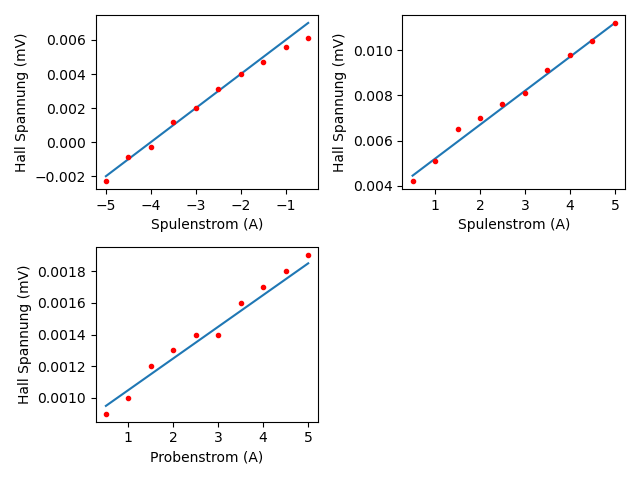
\includegraphics{plothall.png}

In den Koordinatensystemen sind die gemessenen Hall-Spannungen aufgetragen.
Zu den Geaphen ist zu sagen, dass auf der x-Achse entweder der Spulenstrom oder der Probenstrom abgebildet wird.
Die jewils andere Stromstärke wird konstant bei 5A gehalten.

\subsection{Ladungsträger pro Volumen}
Die Ladungsträger pro Volumen berechnen sich nach Formel \ref{Ladungsträger n}:
\begin{center}
    \captionof{table}{Geometrische Abmessungen in cm}
    \begin{tabular}{ll@{${}\pm{}$}lll}
        \toprule
        I\textsubscript{q}[A]&n&Fehler \\
        \midrule
        0.5 &$ -2.608884*10^{31}$&$2.60888*10^{27} $\\
        1   &$  -9.37586*10^{31}$&$9.37586*10^{27}$\\
        1.5 &$  -1.73401*10^{31}$&$-1.734036*10^{28}$\\
        2   &$  -2.89982*10^{31}$&$-2.89982*10^{28}$\\
        2.5 &$  -4.10853*10^{31}$&$4.10853*10^{28} $\\
        3   &$  -5.50691*10^{31}$&$5.50691*10^{28} $\\
        3.5 &$  -6.56558*10^{31}$&$6.565585*10^{28}$\\
        4   &$  -7.80967*10^{31}$&$7.809675*10^{28}$\\    
        4.5 &$  -8.96316*10^{31}$&$8.96316*10^{28} $\\
        5   &$  -1.00170*10^{31}$&$1.001702*10^{28}$\\
        \bottomrule
    \end{tabular}
\end{center}
\section{Ladungsträger pro Atom}

Die Ladungsträger pro Atom berechnen sich nach:

\begin{displaymath} 
    Z= \frac{n*m}{\rho * N_A}
\end{displaymath}
Dabei ist m die molare Masse von Kupfer, $\rho$ ist die Dichte von Kupfer und N\textsubscript{A} ist die Avogadro-Konstante.
$\rho = 8.96$
$m = 63.546e-3$

Die Rechnung ergibt:
\begin{center}
    \begin{tabular}{l @{${}\pm{}$}ll @{${}\pm{}$}l}\\
        \toprule
        Ladungsträger pro Volumen & Gauß-Fehler & Ladungsträger pro Atom & Gauß-Fehler\\
        \midrule
        $-2.6088847454095256*10^{30}$ &  $2.608884745409526 *10^{27} $  &   -30724.4558 &  30.7244\\
        $-9.375861670676898 *10^{30}$  & $9.375861670676899  *10^{27}$    &  -110418.1579 &  110.4181\\
        $-1.7340192518405735*10^{31}$ &  $1.7340192518405736*10^{28} $ &  -204212.9228 &   04.2129   \\   
        $-2.8998249303089926*10^{31}$ &  $2.899824930308992 *10^{28} $  &  -341508.1603 &  341.5081\\
        $-4.108537223356665 *10^{31}$  & $4.108537223356666  *10^{28}$    &  -483856.4474 &   483.8564\\
        $-5.506911710141514 *10^{31}$  & $5.506911710141516  *10^{28}$     &  -648540.9748 &   648.5409\\
        $-6.565587430250072 *10^{31}$  & $6.5655874302500725 *10^{28}$   &  -773219.6731 &   773.2196 \\
        $-7.809670538066778 *10^{31}$  & $7.8096705380667795 *10^{28}$   &  -919733.5295 &    919.7335 \\ 
        $-8.963167117987643 *10^{31}$  & $8.963167117987643  *10^{28}$    &  -1055579.1425 &  1055.5791 \\
        $-1.001706478691359 *10^{32}$  & $1.001706478691359  *10^{29}$   &  -1179695.1366 &  1179.6951 \\
        \bottomrule
    \end{tabular}
\end{center}

\section{mittlere Flugzeit}

Die mittlere Flugzeit berechnet sich nach:

\begin{displaymath}
    \tau = \frac{2m_0}{ne_0^2*\rho}
\end{displaymath}

Die Rechnung ergibt:
\begin{center}
    \begin{tabular}{l @{${}\pm{}$}lll}\\
    \toprule
    Mittlere Flugzeit & Gauß-Fehler\\
    \midrule
    $-3.036*10^{24}$ &  $3.0362*10^{27}$ \\
    $-8.448*10^{25}$ &  $8.4484*10^{28}$ \\
    $-4.568*10^{25}$ &  $4.5681*10^{28}$ \\
    $-2.731*10^{25}$ &  $2.7316*10^{28}$ \\
    $-1.927*10^{25}$ &  $1.9279*10^{28}$ \\
    $-1.438*10^{25}$ &  $1.4384*10^{28}$ \\
    $-1.206*10^{25}$ &  $1.2064*10^{28}$ \\
    $-1.014*10^{25}$ &  $1.0142*10^{28}$ \\
    $-8.837*10^{26}$ &  $8.8374*10^{29}$ \\
    $-7.907*10^{26}$ &  $7.9076*10^{29}$ \\
    \bottomrule
    \end{tabular}
\end{center}


\subsection{Driftgeschwindigkeit}
Die Driftgeschwindigkeit errechnet sich nach
\begin{equation}
    \bar{v_d}=\frac{-n*e_0}{j}
\end{equation}
mit Stromdichte $j=1 A/mm^2$:
\begin{center}
    \captionof{table}{Driftgeschwindigkeit}
    \begin{tabular}{ll}
        \toprule
        Probenstrom (A) & V\textsubscript{d} (m/s) \\
        \midrule  
        0.5       & 417989417989.418+/-417989417.989     \\
        1         &  1502178649237.4727+/-1502178649.237  \\
        1.5       &   2778205128205.128+/-2778205128.2051  \\
        2         &   4646031746031.746+/-4646031746.0317  \\
        2.5       &   6582602339181.287+/-6582602339.1812 \\
        3         &  8823045267489.715+/-8823045267.4897  \\
        3.5       &   10519230769230.77+/-10519230769.230 \\
        4         &   12512471655328.799+/-12512471655.3288    \\
        4.5       &   14360576923076.922+/-14360576923.0769  \\
        5         &   16049107142857.143+/-16049107142.8571   \\
        \bottomrule
    \end{tabular}
\end{center}

\subsection{Beweglichkeit \mu}
Die Beweglichkeit \mu errechnet sich nach der Formel 
\begin{equation}
    \mu=-\frac{e_0}{2m_0}*\tau
\end{equation}
Sie stellt eine Beziehung zwischen \tau und \mu auf.
\begin{center}
    \captionof{table}{Bewglichkeit \mu}
    \begin{tabular}{ll}
        \toprule
        Mittlere Driftgeschwindigkeit & Bewglichkeit \\
        \midrule  
               & 2.6700949367088606e-13+/-2.6700949367088604e-16\\
               & 7.429685071998344e-14+/-7.429685071998343e-17\\
               & 4.017239106071593e-14+/-4.0172391060715934e-17\\
               & 2.4022036214554153e-14+/-2.4022036214554153e-17\\
               & 1.6954866344094545e-14+/-1.6954866344094548e-17\\
               & 1.2649503598081023e-14+/-1.2649503598081026e-17\\
               & 1.060981979629146e-14+/-1.0609819796291459e-17\\
               & 8.919671982602391e-15+/-8.919671982602392e-18   \\
               & 7.771772920751831e-15+/-7.771772920751833e-18 \\
               & 6.9541029207232255e-15+/-6.954102920723227e-18  \\
        \bottomrule
    \end{tabular}
\end{center}
\subsection{mittlere freie Weglänge}

Die mittlere freie Weglänge berechnet sich dur die Formel:

\begin{displaymath}
    l = -\tau * v
\end{displaymath}

Einsetzen der Werte aus den voherigen Rechnungen liefert:

\begin{center}
    \begin{tabular}{l @{${}\pm{}$}lll}\\
    \toprule
    Mittlere freie Weglänge & Gauß-Fehler\\
    \midrule
    2483.064  & 2.483 \\
     690.926  & 0.6909    \\
     373.584  & 0.3735     \\
     223.393  & 0.223 \\
     157.672  & 0.1576  \\
     117.634  & 0.1176 \\
     98.6663  & 0.0986 \\
     82.9488  & 0.0829 \\
     72.2738  & 0.0722  \\
     64.6699  & 0.0646 \\
    \bottomrule
    \end{tabular}
\end{center}

\section{Diskussion}
Die nach den oben beschriebenen Formeln errechneten Werte weichen sehr stark von realistischen oder gar physikalisch möglichen Werten ab. Dabei liegen die Fehler schon zu Beginn der Rechnungen bei sehr großen Werten. Diese Fehler vermehren sich daraufhin gravierend und führen dadurch zu kumalativ immer größer werdenden Fehlern. Es fällt besonders bei den Geschwindigkeiten v\textsubscript{d} und der Totalgeschwindigkeit auf, dass diese mit Werten größer als die Lichtgeschwindigkeit natürlich fern jeder physikalischen Sinnhaftigkeit liegen. Die Vermutung liegt nahe, dass es sich dabei um signifikante Messfehler oder systematische Ungereimtheiten an der Messapparatur handelt, so dass solch großen Fehler möglich werden. Besonders Zweiteres ist wahrscheinlich, da es bei der Durchführung des Versuchs immer wieder Probleme mit dem Teslameter und dem Generator gegeben hat. Auch das Messgerät zur Messung der Hall-Spannung stellte die Messwerte sehr unzuverlässig und mit für die Messwerte sehr großer, relativer Fluktuation dar. Es gab auch zwischendurch immer mal wieder komplette Aussetzer des Messgeräts, in denen es mitten in einer Messreihe plötzlich das Vorzeichen ohne Grund änderte. Diese Umstände erschwerten ein genaues und zuverlässiges Ablesen und Aufnehmen der Messwerte sehr. Außerdem kommt dazu, dass die gemessenen Hall-Spannungen so klein sind, dass selbst ein scheinbar geringer Fehler schon eine signifikante Abweichung bedeutet und dadurch das weitere Rechnen stark beeinflusst. Alles zusammen sorgt dann für die zum Teil abstrusen Ergebnisse.

\section{Messwerte}
\begin{center}
    \captionof{table}{Magnetfeld}
    \begin{tabular}{lll}
        \toprule
        Spulenstrom (A) & B (mT) & B\textsubscript{0}(mT) \\
        \midrule 
        0.001     &      0.3  &   0\\
        0.5       &      63.5 &   63.2 \\
        1         &      138.2&   137.9\\
        1.5       &      217  &   216.7\\
        2         &      293  &   292.7\\
        2.5       &      360.5&   360.2\\
        3         &      429.1&   428.8\\
        3.5       &      492.6&   492.3\\
        4         &      552.1&   551.8\\
        4.5       &      597.7&   597.4\\
        5         &      647.4&   647.1\\
        \bottomrule
    \end{tabular}
\end{center}

\begin{center}
    \captionof{table}{Magnetfeld umgepolt}
    \begin{tabular}{lll}
        \toprule
        Spulenstrom (A) & B (mT) & B\textsubscript{0}(mT) \\
        \midrule 
        0.001     &   -32    & -0 \\
        0.5       &   -95    & -63 \\
        1         &   -169   & -137\\ 
        1.5       &   -244   & -212\\ 
        2         &   -315   & -283\\ 
        2.5       &   -385   & -353\\ 
        3         &   -450   & -418\\ 
        3.5       &   -517   & -485\\ 
        4         &   -572   & -540\\ 
        4.5       &   -628   & -596\\ 
        5         &   -676   & -644\\
        \bottomrule
    \end{tabular}
\end{center}

\begin{center}
    \captionof{table}{Hallspannungen 5A Probenstrom}
    \begin{tabular}{lll}
        \toprule
        Stromstärke Spule (A) & Hall-Spannung (mV) \\
        \midrule 
          0.5      & 0.0042\\
          1        & 0.0051\\
          1.5      & 0.0065\\ 
          2        & 0.007\\ 
          2.5      & 0.0076\\ 
          3        & 0.0081\\ 
          3.5      & 0.0091\\ 
          4        & 0.0098\\ 
          4.5      & 0.0104\\ 
          5        & 0.0112\\ 
        \bottomrule
    \end{tabular}
\end{center}

\begin{center}
    \captionof{table}{Hallspannungen 5A Probenstrom}
    \begin{tabular}{lll}
        \toprule
        Stromstärke Spule umgepolt (A) & Hall-Spannung (mV) \\
        \midrule 
          0.5      &  -0.0023\\
          1        &  -0.0009\\
          1.5      &  -0.0003\\ 
          2        &  0.0012\\ 
          2.5      &  0.002\\ 
          3        &  0.0031\\ 
          3.5      &  0.004\\ 
          4        &  0.0047\\ 
          4.5      &  0.0056\\ 
          5        &  0.0061 \\ 
        \bottomrule
    \end{tabular}
\end{center}

\begin{center}
    \captionof{table}{Hallspannungen 5A Spulenstrom}
    \begin{tabular}{lll}
        \toprule
        Stromstärke Probe (A) & Hall-Spannung (mV) \\
        \midrule 
          0.5      & 0.0009 \\
          1        & 0.001 \\
          1.5      & 0.0012 \\ 
          2        & 0.0013 \\ 
          2.5      & 0.0014\\  
          3        & 0.0014 \\ 
          3.5      & 0.0016 \\ 
          4        & 0.0017 \\ 
          4.5      & 0.0018 \\ 
          5        & 0.0019 \\ 
        \bottomrule
    \end{tabular}
\end{center}

\section{Literaturverzeichnis}
Anleitung V311 Halleffekt und Elektrizitätsleitung bei Metallen: $https://moodle.tu-dortmund.de/pluginfile.php/1368594/mod_resource/content/1/V311.pdf$\\
Literaturwerte für Dichte und molare Masse von Kupfer: $https://www.chemie.de/lexikon/Kupfer.html$\\
SciPy-Bibliothek für Naturkonstanten (Python-Erweiterung)
\end{document}